\chapter{方法设计}
\label{chap:algorithm}

\section{棋盘规则}
超级皇后的棋盘继承国际象棋的规格,并且可以根据喜好扩大盘面(8x8,12x12,16x16等等)。在我们设计的API中,游戏开始时棋盘的大小可以任意自定义。受限于设备,AlphaZero框架的AI玩家只训练了8x8棋盘(经典棋盘)。因此在本文中我们主要关心8x8棋盘的结果。
超级皇后对战的规则也可以在我们设置的api中指定,如引言中所述,超级皇后走法规则可选三个规则:(1)超级状态(super),拥有皇后和骑士的权限,可按此两种棋子落子规则任意移动;(2)皇后状态(queen),可横竖对角线移动,不可越过移动直线上的对手;(3)骑士状态,可走“日”字,即先向左(或右)走1格,再向上(或下)走2格;或先向左(或右)走2格,再向上(或下)走1格。
棋盘每个位置都具有四个状态值候选:$\{white:1, black:-1,empty:0,dead:99\}$,抛开初始位置(左上角与右下角),剩余位置的状态转换如下所示:
\begin{equation}
    \begin{aligned}
    empty &\stackrel{\mathrm{move}}{\longrightarrow} black \stackrel{\mathrm{leave}}{\longrightarrow} dead \\
     &\stackrel{\mathrm{move}}{\longrightarrow} white \stackrel{\mathrm{leave}}{\longrightarrow} dead 
    \end{aligned}
\end{equation}

依据信息暴露程度,超级皇后对战属于完美信息游戏(Perfect-Information Game)\cite{binmore2007game}。对于完美信息游戏,可以用状态空间复杂度(State-Space Complexity)和博弈树复杂度(Game-Tree Complexity)对其难度进行衡量\cite{allis1994searching,VANDENHERIK2002277}。
状态空间复杂度是指从初始状态开始,可以实现的所有符合规则的状态的集合总数,在实际情况中一般使用该数量的上界表示,例如在围棋中允许出现全白或全黑的极端情况。
博弈树复杂度表示所有不同游戏路径数目,常用合理估计的下界表示:$valids^{turn}$。 $valids$表示每回合平均合法移动数目,$turn$表示平均游戏长度。
类似于国际象棋与围棋,我们可以给出超级皇后对战的状态空间与博弈树复杂度(仅考虑8x8棋盘):
\begin{figure}[htb]
    \centering
    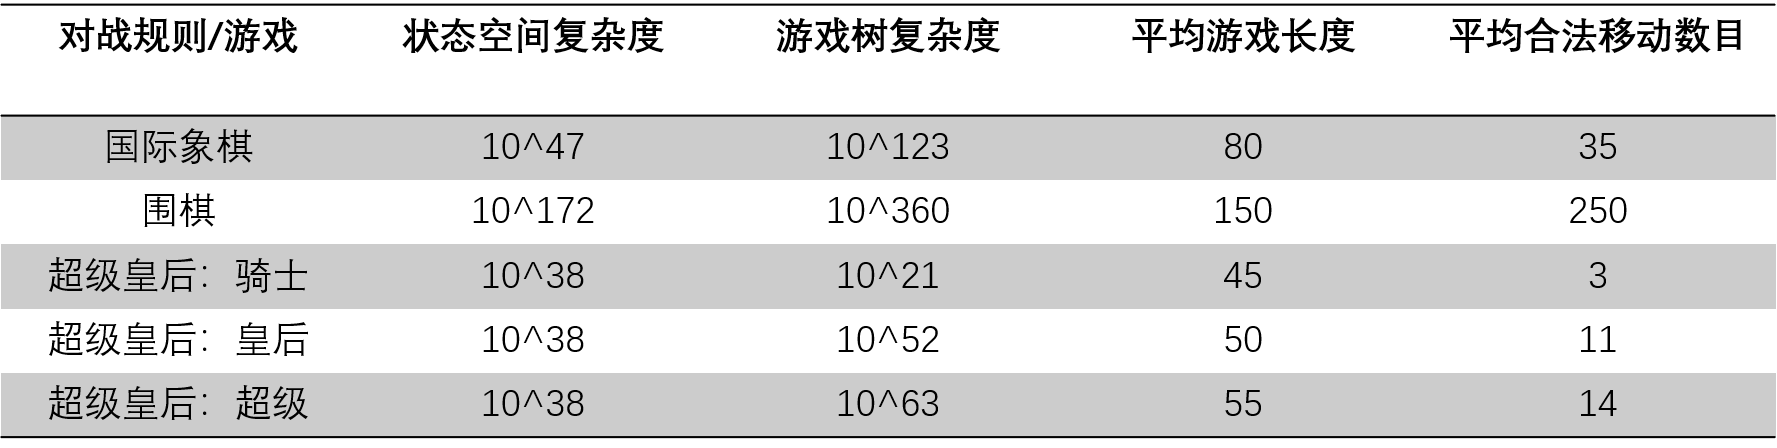
\includegraphics[width=1\textwidth]{complexity.png}
    \caption[complexity]{%
        超级皇后对战复杂度\cite{enwiki:complexity}%
      }
    \label{fig:complexity}
\end{figure}

\begin{figure}[htb]
    \centering
    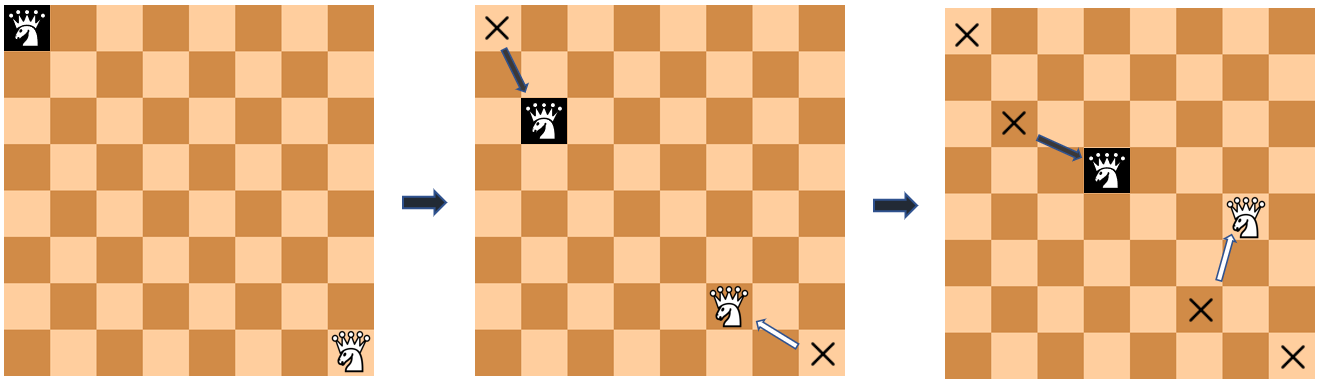
\includegraphics[width=0.8\textwidth]{knight.PNG}
    \caption[rules-knight]{%
        超级皇后对战游戏规则——骑士状态%
      }
    \label{fig:knight}
\end{figure}

\begin{figure}[htb]
    \centering
    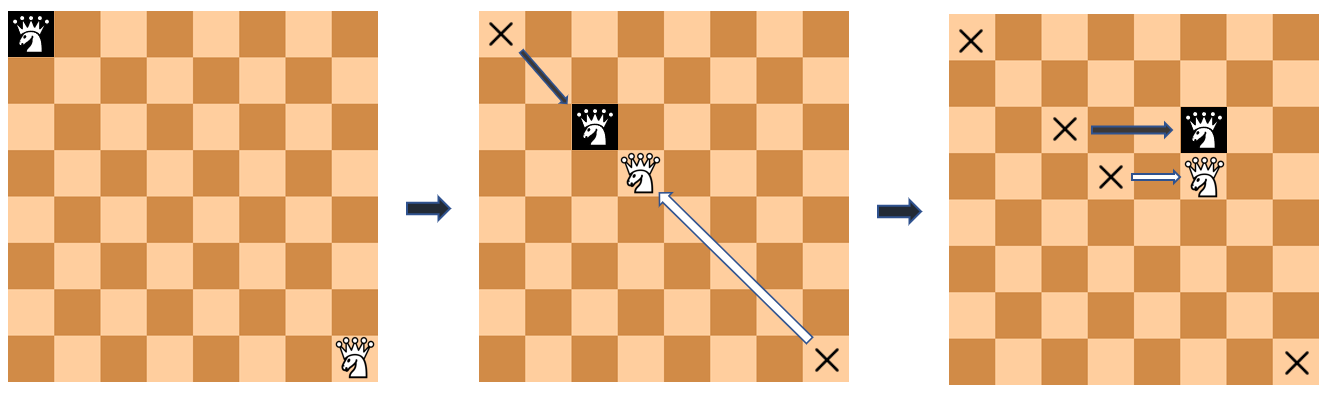
\includegraphics[width=0.8\textwidth]{queen.PNG}
    \caption[rules-queen]{%
        超级皇后对战游戏规则——皇后状态%
      }
    \label{fig:queen}
\end{figure}

\begin{figure}[htb]
    \centering
    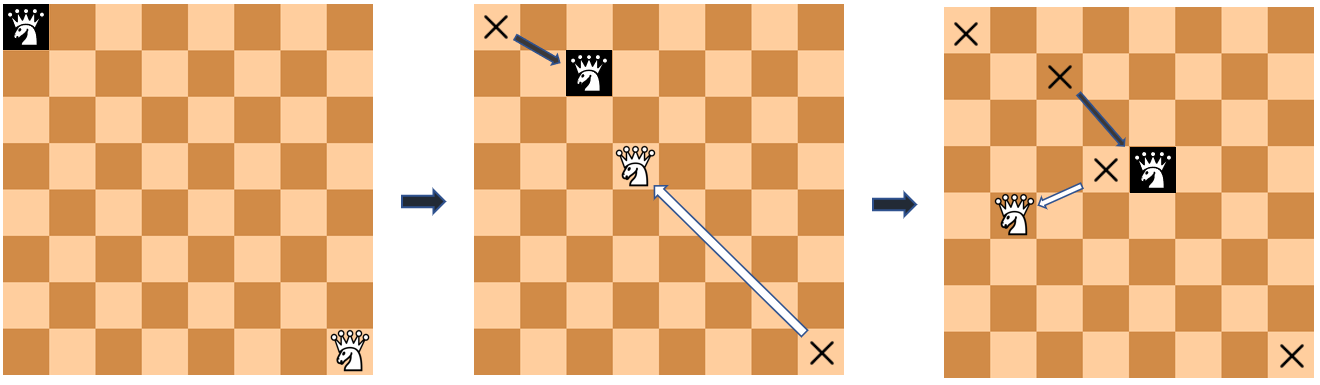
\includegraphics[width=0.8\textwidth]{super.PNG}
    \caption[rules-super]{%
        超级皇后对战游戏规则——超级状态%
      }
    \label{fig:super}
\end{figure}
骑士状态下,不论是Alpha-beta剪枝还是蒙特卡洛树搜索进行模拟速度都相对较快,因此在自我对弈阶段的落子速度也很快,但由于博弈树复杂度较低,启发式搜索算法的效果可能会好于基于蒙特卡洛树搜索的AlphaZero框架,因为其可以在较短时间内较小深度下搜索大部分个博弈树,其局部最优解更靠近全局最优解。
而超级状态下每回合平均合法移动数目相对较多,搜索代价较大,在同等限制下更加适合深度强化学习AlphaZero训练出的模型。

\section{数据生成}

\section{学习过程}

\subsection{蒙特卡洛树搜索}

\subsection{策略网络与值网络}